\documentclass[12pt,letterpaper]{article}

% just for the example
\usepackage{lipsum}
% Set margins to 1.5in
\usepackage[margin=1.5in]{geometry}

\usepackage{url}

\usepackage{enumitem}

% for graphics
\usepackage{graphicx}
\graphicspath{{./figures/p3/}}

% for crimson text
\usepackage{crimson}
\usepackage[T1]{fontenc}

% setup parameter indentation
\setlength{\parindent}{0pt}
\setlength{\parskip}{6pt}

% for 1.15 spacing between text
\renewcommand{\baselinestretch}{1.15}

% For defining spacing between headers
\usepackage{titlesec}
% Level 1
\titleformat{\section}
  {\normalfont\fontsize{18}{0}\bfseries}{\thesection}{1em}{}
% Level 2
\titleformat{\subsection}
  {\normalfont\fontsize{14}{0}\bfseries}{\thesection}{1em}{}
% Level 3
\titleformat{\subsubsection}
  {\normalfont\fontsize{12}{0}\bfseries}{\thesection}{1em}{}
% Level 4
\titleformat{\paragraph}
  {\normalfont\fontsize{12}{0}\bfseries\itshape}{\theparagraph}{1em}{}
% Level 5
\titleformat{\subparagraph}
  {\normalfont\fontsize{12}{0}\itshape}{\theparagraph}{1em}{}
% Level 6
\makeatletter
\newcounter{subsubparagraph}[subparagraph]
\renewcommand\thesubsubparagraph{%
  \thesubparagraph.\@arabic\c@subsubparagraph}
\newcommand\subsubparagraph{%
  \@startsection{subsubparagraph}    % counter
    {6}                              % level
    {\parindent}                     % indent
    {12pt} % beforeskip
    {6pt}                           % afterskip
    {\normalfont\fontsize{12}{0}}}
\newcommand\l@subsubparagraph{\@dottedtocline{6}{10em}{5em}}
\newcommand{\subsubparagraphmark}[1]{}
\makeatother
\titlespacing*{\section}{0pt}{12pt}{6pt}
\titlespacing*{\subsection}{0pt}{12pt}{6pt}
\titlespacing*{\subsubsection}{0pt}{12pt}{6pt}
\titlespacing*{\paragraph}{0pt}{12pt}{6pt}
\titlespacing*{\subparagraph}{0pt}{12pt}{6pt}
\titlespacing*{\subsubparagraph}{0pt}{12pt}{6pt}

% Set caption to correct size and location
\usepackage[tableposition=top, figureposition=bottom, font=footnotesize, labelfont=bf]{caption}

% set page number location
\usepackage{fancyhdr}
\fancyhf{} % clear all header and footers
\renewcommand{\headrulewidth}{0pt} % remove the header rule
\rhead{\thepage}
\pagestyle{fancy}

% Overwrite Title
\makeatletter
\renewcommand{\maketitle}{\bgroup
   \begin{center}
   \textbf{{\fontsize{18pt}{20}\selectfont \@title}}\\
   \vspace{10pt}
   {\fontsize{12pt}{0}\selectfont \@author} 
   \end{center}
}
\makeatother

% Used for Tables and Figures
\usepackage{float}

% For using lists
\usepackage{enumitem}

% For using APA Citation format
\usepackage{apacite}

% Custom Quote
\newenvironment{myquote}[1]%
  {\list{}{\leftmargin=#1\rightmargin=#1}\item[]}%
  {\endlist}
  
% Create Abstract 
\renewenvironment{abstract}
{\vspace*{-.5in}\fontsize{12pt}{12}\begin{myquote}{.5in}
\noindent \par{\bfseries \abstractname.}}
{\medskip\noindent
\end{myquote}
}

\begin{document}

% Set Title, Author, and email
\title{Assignment P5}
\author{Snejana Shegheva \\ sshegheva3@gatech.edu}

\maketitle
\thispagestyle{fancy}

\section*{Question 1 - Intersection of Technology and Society}

\textit{Our teaching assistants are the lifeblood of this program} - writes David Joyner on one of his emails inviting applications for TA in the OMSCS program. 

Teaching Assistants play an essential role in education across all universities, especially the large ones. For a program like OMSCS, that is 100\% remote, the availability of qualified and motivated TAs is even more paramount. Who could have predicted that not only would enough applicants be willing to contribute, but their applications would be turned away due to overabundance?

The sheer number of TAs with vast experience across many backgrounds who are eager to contribute to a greater education appeared as an \textbf{unexpected positive effect}. My personal skepticism about the success of the program due to its scale and remoteness dissolved primarily as a result of my interactions with the TAs from the very beginning of the program. 

Due it its low cost, the OMSCS program attracted a tremendous number of students to the Computer Science field. The sudden accessibility of classes from Computer Science department might be potentially having a \textbf{negative repercussion} for other departments. I do not have data to substantiate my conclusions, but drawing from my personal experience, I could say that \textit{CS availability} factor played a significant role in my decision making when applying to a Master's Program. If all programs at GaTech had been equally available, the school of Mathematics would have been my first choice. It would be interesting to forecast a number of students in other departments if they would have a similar program and compare it with OMSCS.  

It is understandable that OMSCS was a pilot program, and more are expected to be added soon (Online Masters in Analytics has already followed). A great way to \textbf{reduce} the described drawback is to include more \textbf{electives} in the program from \textbf{different departments}, such as Mathematics, Music, Philosophy, etc. This addition would serve as a bridge to other fields that do not yet offer a similar program. Increasing the coverage of classes will likely not impinge current positive experiences in the program.

\section*{Question 2 - Political Motivations}

The field of Artificial Intelligence-based Medical Diagnosis Support System (AIMDSS) has been gaining considerable momentum due to significant advances in Artificial Intelligence (AI) imaging technologies and Natural Language Processing (NLP) techniques. Multiple studies into the adoption of such a system by health professionals focus on various factors that impact their general acceptability \cite{fan2018investigating}.

There are many \textbf{stakeholders} (direct and indirect) in this area, and here we are identifying three main groups:

\begin{itemize}
    \item AI Researchers
    \item Healthcare Professionals
    \item Patients 
\end{itemize}

The \textbf{motivations} for \textbf{patients} include \textbf{safety} and \textbf{accuracy} of the diagnostic tools powered by AI. As algorithms are getting integrated into the diagnostic methods, it is important that the results of automated processes are sufficiently trustworthy and carry a minimum risk to the patient's health. 

\textbf{Healthcare professional's} incentives include increasing their \textbf{clinical productivity}, \textbf{safety} for use and \textbf{user-friendliness} in operating the systems \cite{ishak2002artificial}. An AI system that is not easily interpretable will face many challenges in adoption even if the healthcare professionals are well-intentioned in adopting it in their routines. 

\textbf{AI researches} are inspired by \textbf{advancing} the fields of machine learning, deep learning, natural language processing, and other AI-related fields. Therefore their motivations are in part driven by developing the next generation tools that bring exciting breakthroughs to the area of patients' care.

The design of Augmented Intelligence for Healthcare is influenced by all groups even beyond those identified above. When AI researches drive the evolution of AI decision-making tools, they primarily focus on the technical challenges, such as parsing massive records of unstructured patient's data or classifying images based on large volumes of training data. As their algorithms start to permeate the industry fields outside of Academic's world, it is crucial that they address \textbf{ethical} and \textbf{privacy issues} for the patients. The conditions for adoption must include validation that algorithms are free of bias and meet the transparency levels that satisfy \textit{thoughtfully designed, high-quality, clinically validated healthcare AI} \cite{blog:healthitanalytics}.

Healthcare professionals might find the emergence of AI tools for healthcare potentially disruptive to the traditional healthcare community. \textbf{Integration} and \textbf{deployment} has been at the forefront of challenges in adoption of AI tools. The professional society must continue to influence the design of such tools to meet the criteria of user-friendliness \cite{heathfield1993philosophies}. To comfortably work with AI tools, physicians must acquire skills for interpreting the results of the AI system. If such systems are not designed with the user in mind, the integration will continue to fail. 

Patients are one of the principal stakeholders; therefore their involvement in the evolution of the AI systems in healthcare is of extreme importance. Users must drive the goals behind the design of tools for healthcare. Society can better benefit from technologies when questions "What can the computer do?" are replaced with \textbf{"What can people do?"} \cite{hesse2007ehealth}. By taking an active role and encouraging the researches to ask the right questions, patient-centered perspective gains emphasis in the design of the augmented systems. 

\section*{Question 3 - Piazza Post Filtering Redesign}

As a candidate for re-design, I selected Piazza's functionality on \textbf{filtering posts} based on the user's preference to prioritize the selection. Figure~\ref{fig::1} demonstrates the new design that focuses on making a post-reading activity more efficient. 

\textbf{Explaining the Mock-up}. Current Piazza interface provides an ability to filter messages by categories such as \textit{Unread}, \textit{Updated}, \textit{Unresolved}, etc. The idea behind the re-design is 1) \textbf{augmenting} the available selections with visual representation of post statistics and 2) \textbf{changing} the existing categories by adding \textit{Read} and \textit{Authored by me} and removing \textit{Updated}, \textit{Unresolved}, \textit{Due to Answer} and \textit{Archived}.

Each category in the filtering set is captured statistically by counting a frequency of posts in the category aggregated by a certain period of time (for example weekly). The goal of the visualizations is to identify and communicate trends for participant's behavior, students or instructors. With the addition of charts, some of the categories are removed to avoid the clutter leaving only the more essential filters. 


\begin{figure}[h]
\centering
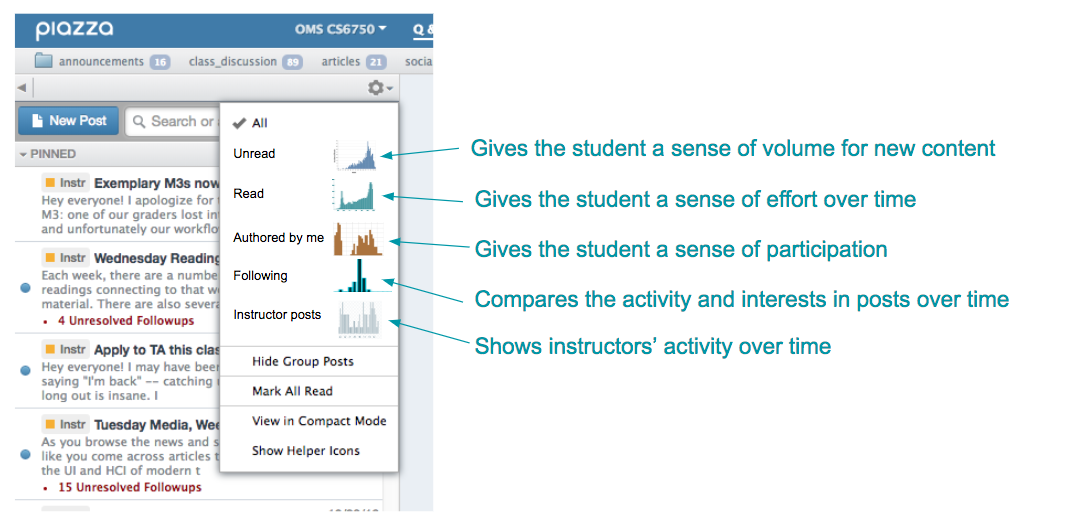
\includegraphics[scale=.5]{figures/p5/piazza_filtering.png}
\caption{Mock-up for Piazza Filtering Functionality redesign}
\label{fig::1}
\end{figure}

\subsection*{Justifying the Redesign}

\textbf{Cognitive Load}. An important aspect of designing a good interface is planning a task execution that reduces the user effort or requires a minimal cognitive load that is not related to the task itself. When a user logs into Piazza, they need to optimize their cognitive efforts for reading and digesting the material. Finding the right content should not be time-consuming; therefore a good design must guide the user through the interface that de-emphasizes the clutter and off-loads tasks that require heavy user processing onto the interface. How does the Piazza user know if they are staying on top of reading the new content? Currently, they have to scroll down the list of posts and count how many of them have a \textit{blue-dot} that indicated the unread material. Alternatively, they can see counts of posts in each folder, such as \textit{announcements}, \textit{class discussions}, etc. The new design accessed via filtering functionality gives the user a sense of volume of read/unread posts. A student may use this information to adjust their learning habits as needed, for example, visit Piazza more frequently.     

\textbf{Perception in the Gulf of Evaluation}. The new design communicates information on the rate of incoming Piazza posts effectively by aggregating their frequencies over time. The user stays informed about the pattern of content creation through the visual feedback represented with histograms over time. If the user's goal is to keep up with Piazza's updates, they can easily bridge the gulf of evaluation via perception stage that helps determine if their intentions have been met. The student can assess the new state of Piazza posts and decide how to divide their focus between categories.

\textbf{Flexibility Heuristic}. The selection of current filters does not address potential user's preferences to narrow down Piazza's content to their posts with an intention to review the comments in responses. The new design adds categories for \textit{Read} and \textit{Authored by me} posts to remove the limitation. Ideally, the user could customize their filters in the advanced mode (not shown in the mock-up) to fit their individual interaction habits. 

\textbf{Representation in Interfaces}. The new re-design of the filtering functionality gives a representation of the student's pace in the class. For example, by showing a weekly count of read posts (with the histogram icons), the student can get a sense for how consistent they are in keeping up with the new content. The new design also provides a good representation at a glance for how much they contribute, and how does the latest pattern compare with their past habits. An interface with a representation of the user's activity has the power to change user behavior. 

\textbf{Simplicity}. By removing certain categories from the filter set, we reduce the options that are rarely used. A minimal set can be easily decided by sending out a survey asking users to estimate how relevant is each option to them. The new design intentionally sets visible filters  (with the corresponding visualization) to five that would make the interface simpler and more intuitive to use. The simplicity principle is implemented by focusing on the most common filters that may or may not be in the original set of filters. Requesting feedback from the user during interface design iterations can help highlight the important information for the accurate interpretation of the current Piazza activity.

\section*{Question 4 - Paper Distillation}

\textbf{Title}: Increasing User's Confidence in Uncertain Data by Aggregating Data from Multiple Sources \cite{greis2017increasing}

The authors perform a compelling study on how to help users make more informed decisions in the context where there is no sufficient trust in a single source of data. With a goal to reduce the cognitive load for having to compare multiple sources manually, they identify and evaluate a few different \textbf{aggregation mechanisms}. They seek to understand what information can be useful for \textbf{the user} to increase their confidence in decision making. 

What does it mean when the data is \textit{uncertain}? 

When interpreting the data from a \textbf{single} source, the concept of uncertainty is typically related to statistical uncertainty, such as noisy or anomalous measurements. In this paper, however, the data uncertainty implies the presence of inconsistencies and even conflicts between \textbf{multiple} sources. For example, one weather app may show that it will rain tomorrow, while another app promises a sunny day. If you are planning a hiking trip, the confidence in the forecast is essential in making a decision on what gear to take, or whether or not to cancel the trip.  

Is there a gap between service providers and user in terms of trust? Yes. The research shows that the general public does not have an intuitive understanding of probabilities, so the service providers, who attempt to quantify the uncertainty, frequently fail in increasing the user's trust in data.

So, what do the users want? 

According to the two experiments performed by the authors - online survey and an alternative interface designed for comparison - users prefer 1) \textbf{Transparency} that can inform their decisions 2) \textbf{Control} (or a feeling of control) over decisions. The experiments were designed to estimate user's trust in data in three different setups of data aggregation - direct comparison, aggregating with ranges, aggregating by averaging. 

What are the implications to the interface designers (in applications with uncertain data)?

\hspace{10mm} - Give users control by \textbf{supporting contexts} with different importance. The survey results showed that users prefer more manual/direct comparison in high-stake situations, such as financial decisions. Giving users the ability to choose different context allows them to make a judgment on how to view and compare data from multiple sources.  

\hspace{10mm} - Anticipate \textbf{different types of users}. The applications should allow users to choose a method of interaction that is suitable to their individual preferences. Some users may choose to tolerate certain levels of uncertainty and use methods that require less mental efforts for interpretation. Other users may prefer an advanced view with options to customize the aspects of their interactions. 

\hspace{10mm} - Establish \textbf{transparency}. Help the user understand the reasoning given by the interface. For example, a service for aggregating news feeds may include the details on the original sources and explanation on how the data has been aggregated. 

The authors of the paper conclude that user's confidence in data \textbf{increases} with additional sources independently of its representation - pictograms, graphs, or text. The comprehension of data changes with the level of aggregation, therefore transparency and flexibility are paramount for gaining user's trust in the scenarios with uncertain data. 

\bibliographystyle{apacite} 
\bibliography{bibtemp}

\end{document}
